\documentclass[a4paper]{oblivoir}
\usepackage{amsmath,amssymb,kotex,kswrapfig,mdframed,paralist}
\usepackage{fapapersize}
\usefapapersize{210mm,297mm,20mm,*,20mm,*}

\usepackage{tabto,pifont}
\TabPositions{0.2\textwidth,0.4\textwidth,0.6\textwidth,0.8\textwidth}
\newcommand\tabb[5]{\par\noindent
\ding{172}\:{\ensuremath{#1}}
\tab\ding{173}\:\:{\ensuremath{#2}}
\tab\ding{174}\:\:{\ensuremath{#3}}
\tab\ding{175}\:\:{\ensuremath{#4}}
\tab\ding{176}\:\:{\ensuremath{#5}}}

\usepackage{graphicx}

%\pagestyle{empty}

%%% Counters
\newcounter{num}

%%% Commands
\newcommand\prob[1]
{\vs\bigskip\bigskip\par\noindent\stepcounter{num} \textbf{문제 \thenum) #1}\par\noindent}

\newcommand\pb[1]{\ensuremath{\fbox{\phantom{#1}}}}

\newcommand\ba{\ensuremath{\:|\:}}

\newcommand\vs[1]{\vspace{40pt}}

\newcommand\an[1]{\bigskip\par\noindent\textbf{문제 #1)}\par\noindent}

%%% Meta Commands
\let\oldsection\section
\renewcommand\section{\clearpage\oldsection}

\let\emph\textsf

\begin{document}
\begin{center}
\LARGE준영, 미니테스트 20
\end{center}
\begin{flushright}
날짜 : 2017년 \(\pb3\)월 \(\pb{10}\)일 \(\pb{월}\)요일
,\qquad
제한시간 : \pb{17년}분
,\qquad
점수 : \pb{20} / \pb{20}
\end{flushright}

%
\prob{}
\(\int(6x^2+ax-1)\,dx=bx^3+4x^2+cx+C\)일 때, 상수 \(a\), \(b\), \(c\)의 합 \(a+b+c\)의 값은?
(단, \(C\)는 적분상수)
\tabb9{10}{11}{12}{13}

%
\prob{}
모든 실수 \(x\)에 대하여
\[\frac d{dx}\int(ax^2+4x+b)\,dx=4x^2+cx+5\]
를 만족시키는 상수 \(a\), \(b\), \(c\)의 합 \(a+b+c\)의 값은?
\tabb9{10}{11}{12}{13}

%
\prob{}
다항함수 \(f(x)\)의 도함수가 \(f'(x)=2x-1\)이고 \(f(x)\)의 최솟값이 \(2\)일 때, \(f(2)\)의 값은?
\tabb{\frac{15}4}{4}{\frac{17}4}{\frac92}{\frac{19}4}


%
\prob{}
\begin{minipage}{0.6\textwidth}
함수 \(f(x)\)의 도함수 \(y=f'(x)\)의 그래프가 그림과 같다.
\(y=f(x)\)의 그래프가 \(x\)축에 접할 때, \(f(-1)\)의 값은?
\end{minipage}
\begin{minipage}{0.3\textwidth}
\centering
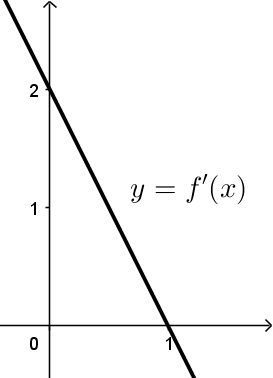
\includegraphics[width=0.5\textwidth]{y=-2x+2}
\end{minipage}
\tabb{-1}{-2}{-3}{-4}{-5}

%
\prob{}
함수 \(\displaystyle f(x)=\int\frac{x^3-1}{x^2+x+1}\,dx+\int\frac{x^3+1}{x^2-x+1}\,dx\)에 대하여 \(f(0)=1\)일 때, \(f(2)\)의 값은?
\par\bigskip
\tabb45678

%
\prob{}
함수 \(f(x)=\int(4ax+1)\,dx\)에 대하여 곡선 \(y=f(x)\) 위의 점 \((1,2)\)에서의 접선의 기울기가 \(5\)일 때, \(f(2)\)의 값은?
(단, \(a\)는 상수이다.)
\tabb56789

%
\prob{}
미분가능한 함수 \(f(x)\)가 모든 실수 \(x\), \(y\)에 대하여
\[f(x+y)=f(x)+f(y)-1\]
을 만족시키고 \(f'(0)=1\)일 때, \(f(10)\)의 값을 구하시오.
\tabb{10}{11}{12}{13}{14}

%
\prob{}
다항함수 \(f(x)\)가 \(f(x)=\frac d{dx}\int_a^x(2t^2+3t)\,dt\)일 때, \(f'(-2)\)의 값은?
(단, \(a\)는 상수이다.)
\tabb{-5}{-4}{-3}{-2}{-1}

%
\prob{}
\(\displaystyle\int_0^1x^2(4x+1)\,dx\)의 값은?
\par\bigskip
\tabb{\frac23}{\frac56}{1}{\frac76}{\frac43}

%
\prob{}
\(\displaystyle\int_0^2(3x^2+1)\,dx+4\int_0^2(x-x^2)\,dx\)의 값은?
\par\bigskip
\tabb{\frac{14}3}{\frac{16}3}6{\frac{20}3}{\frac{22}3}

%
\prob{}
\(\displaystyle\int_0^2|2x-6|\,dx\)의 값은?
\par\bigskip
\tabb{10}{11}{12}{13}{14}

%
\prob{}
\(\displaystyle\int_{-1}^0(x^3+3x^2+2x+4)\,dx+\int_0^1(x^3+3x^2+2x+4)\,dx\)
의 값은?
\par\bigskip
\tabb89{10}{11}{12}

%
\prob{}
\(\displaystyle\lim_{h\to0}\frac1h\int_1^{1+2h}(3x^2-2x+1)\,dx\)의 값은?
\par\bigskip
\tabb2{\frac52}3{\frac72}4

%
\prob{}
\(\displaystyle\lim_{n\to\infty}\sum_{k=1}^n\left(2+\frac{3k}n\right)^2\frac1n=\frac13\int_2^ax^2\,dx\)를 만족시키는 양수 \(a\)의 값은?
\par\bigskip
\tabb34567

\end{document}